


% Contributors: Sam Denton, Jonah Deykin
\section{Hierarchical Clustering}

\subsection{Introduction}
Now that we have discussed the traditional clustering problem, as well as a few algorithms to help solve some of its variants, we will now discuss another type of clustering, hierarchical clustering.  As the name implies, hierachical clustering returns a hierarchy of clusters over a given dataset as opposed to a single partition.  This hierarchy can be thought of as a tree, where all leaf nodes are individual data points and every other node represents a cluster.  This tree then induces a single partition for any given "level", with each partition being a memeber of the hierarchy.   An example of a hierachical clustering is shown below, with the partition induced by the tree at a specific "level" shown by the red line.

\begin{figure}[h]
\centering
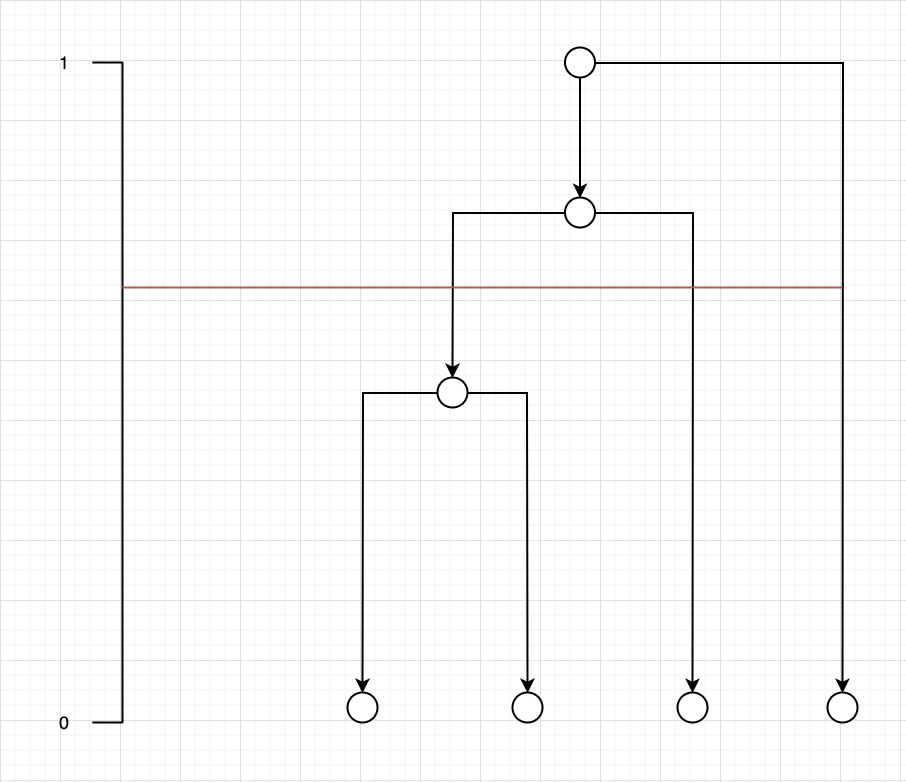
\includegraphics[width=0.7\textwidth]{chapter_1/files/hier_tree_example}
\caption{Visualize hierarchical clustering tree}
\end{figure}

In general, there are two different types of approaches that algorithms which produce heirahircal clustering trees solve.  These two approaches are known as 
\begin{enumerate}
\item \underline{Agglomerative} or "bottom-up" approaches
\item \underline{Divisive} or "top-down" approaches
\end{enumerate}

Both approaches flow intuitively from their names.  Agglomerative ("bottom-up") methods start out by treating each data point as its own cluster, then clusters are successively merged according to the algorithm until the complete tree has been formed.  Divisive ("top-down") methods on the other hand start with the entire data set as once cluster, and recursively break the clusters into smaller clusters until each observation is its own cluster and the tree is complete.




\subsection{Convergence}
Now that we have defined hierarchical clustering and given a brief overview, it is important to ask what does this clustering tell us about the underlying distribution from which that data is sampled.  More specifically, we would want to know if as the number of sampled data points increases, does the cluster tree returned by some algorithm converge to the "true" cluster tree of the underlying distribution as the number of points sampled goes to $\infty$.

\subsubsection{Definitions}
It is first important to clarify mathematically with respect to what we are defining the convergence rate.  Let us first say $X \subseteq \bbR^d$ and let us define a density distribution over $X$, denoted as $f$.  Now we can define a  $\lambda$ density cluster over $X$  in the following way. 
\begin{definition}[$\lambda$ density cluster ]

 a $\lambda$ density cluster Z over G is a connected component $Z \subseteq X$ such that $\forall z \in Z, f(z) \geq \lambda$.  
 \end{definition}

 We then define the cluster tree of $X$ in the following way
 \begin{definition}[Cluster Tree]
  let us define the cluster tree as $C_f$, where $C$ is a function $C(\lambda)$ = the set of all disjoint connected components such that each component is a $\lambda$ density cluster over $X$. 
 \end{definition} 
 Now let us consider the set \{$X_1, ... X_n\} \subset X$, and let us say using it we construct a tree $C_n$, which is an approximation of $C_f$.  We now can define "consistency" w.r.t $C_n$.  

\begin{definition}[Consistency]
 We say that if $\forall, A, A' \subset X$, let $A_n$ be the smallest cluster from $C_n$ containing $A \cap X_n$, and $A'_n$ be the smallest cluster from $C_n$ containing $A' \cap X_n$, then if $C_n$ is consistent, whenever $A, A'$ are different $\lambda$ density clusters in $X$ for some $\lambda$, $\Pr(A_n$ disjoint from $A'_n) \rightarrow 1$ as $n \rightarrow \infty$.  
 \end{definition}

 We can now express that we are to establish a convergence rate with respect to $n$, the number of samples drawn form $X$ as it relates to the quality of $C_n$, the estimate of $C_f$ constructed from $\{X_1, ... X_n\}$


\subsubsection{Algorithm}
In this section we will define the algorithm used to produce $C_n$ using the sample set $\{X_1, ... X_n\}$.  First let us define $B(x,y)$ as the euclidean ball centered as $x$ with radius $y$. The algorithm depends on two parameters, $k ,\alpha$, and works in the following way
\begin{algorithm}[H]
\caption {Algorithm to produce a cluster tree given samples \{$X_1 ... X_n$\}}
\begin{algorithmic}
\FORALL {$X_i \in \{X_1,...,X_n\}$} 
  \STATE let $r_k(X_i)$ = inf\{$r$ : B($X_i$
, $r$) contains $k$ data points\}
\ENDFOR
\FOR {$r$ from 0 to $\infty$}

    \STATE graph $G_r$ = ($V,E$), where $V$ =  \{$X_i$
: $r_k(X_i) \leq r\}$, $E = \{(X_i, X_j): X_i, X_j \in \{X_1,...X_n\}, \|X_i -X_j \| \leq \alpha r\}$, where $\|.\|$ is the euclidean norm
    \STATE $C_n(r) =$ \{connected components of $G_r\}$
\ENDFOR
\end{algorithmic}
\end{algorithm}

Now let us define a notion of a buffer zone around clusters which the algorithm find.  This buffer is used as given a small sample it is possible for one connected component where two parts are connected by a small segment to have been accidentally labeled as two different connected components.  

\vspace{\baselineskip}
\begin{definition}[$Z_{\sigma}$]
Let $Z \subset \bbR^d$ and $\sigma > 0$.  Then $Z_{\sigma}$ = \{$y \in \bbR^d :$ inf$_{z \in Z}\|y-z\| \leq \sigma\}$
\end{definition}
\vspace{\baselineskip}

Now let us define a notion of separateness of two sets in $X$ using the previous definition. 

\vspace{\baselineskip}
\begin{definition}[Separateness]
Given a density $f$ over $X$, and $A, A' \subset X$ We say that $A, A'$ ($\sigma, \epsilon$)-separated if there
exists $S \subset X$ such that:
\begin{itemize}
  \item Any path in $X$ from $A$ to $A'$
intersects $S$
  \item sup$_{x \in S_{\sigma}} f(x) \leq (1 - \epsilon)$ inf$_{x \in A \cup A'}f(x)$
\end{itemize}
\end{definition}

\vspace{\baselineskip}
Now using these definition we will state the main theorem regarding convergence rates to be proven later.

\vspace{\baselineskip}
\begin{theorem}
There is a $C$, such the for any $\delta, \epsilon > $  0, run the algorithm above on sample $y$ of size $n$ drawn from $f$, with $\sqrt{2} \geq \alpha \geq 2$ and $k$ = $C* \frac{d \-\ log \-\ n}{\epsilon^2}* log^2 \frac{1}{\delta}$ There is a mapping $r: [0, \infty) \rightarrow [0, \infty)$ such that that following hold with probability 1 - $\delta$:

If $A, A'$ are $(\sigma, \epsilon)$ separated and $\lambda = $ inf$_{x\in A_{\sigma} \cup A'_{\sigma}}f(x) \geq \frac{1}{v_d(\frac{\sigma}{2})^d} * \frac{k}{n}*(1+\frac{\epsilon}{2})$

Where $v_d$ is the volume of the unit ball in $\bbR^d$, then 
\begin{itemize}
  \item  Separation: $A \cap X_n$ is disconnected from $A' \cap X_n$ in $G_{r(\lambda)}$
  \item Connectedness: $A \cap X_n$ and $A' \cap X_n$ are each connected in $G_{r(\lambda)}$
\end{itemize}
\end{theorem}

\subsubsection{Separation}
We first start the proof of separation by establishing 3 facts about the relationship between $f$ the actual density underlying $X$, and $f_n$ the empirical density derived from sample $X_n$:

Given $k \geq d$ log $n$.  For every $\delta \geq 0$ there is a constant $C_{\delta}$ such that with probability 1 - $\delta$ the following holds for every ball $B \in \bbR^d$

\begin{itemize}
  \item  $f(B) \geq \frac{C_{\delta} d \-\ log \-\ n}{n} \rightarrow f_n(b) \geq 0$
  \item $f(B) \geq \frac{k}{n} + \frac{C_{\delta}}{n}\sqrt{kd \-\ log \-\ n} \rightarrow f_n(b) \geq \frac{k}{n}$
  \item $f(B) \leq \frac{k}{n} - \frac{C_{\delta}}{n}\sqrt{kd \-\ log \-\ n} \rightarrow f_n(b) < \frac{k}{n}$
\end{itemize}


Then, given we pick $r$, such that $0 < r < \frac{2\sigma}{\alpha+2}$, and 
\begin{itemize}
  \item $v_dr^d\lambda \geq \frac{k}{n} + \frac{C_{\delta}}{n}\sqrt{kd \-\ log \-\ n}$
  \item $v_dr^d(1-\epsilon)\lambda \leq \frac{k}{n} - \frac{C_{\delta}}{n}\sqrt{kd \-\ log \-\ n}$
\end{itemize}
then with probability $> 1-\delta$

\begin{enumerate}
    \item \begin{lemma} graph $G_r$ contains all points in $(A_{\sigma-r} \cup A'_{\sigma-r}) \cap X_n$ and no points in $S_{\sigma - r } \cap X_n$
    \end{lemma}
    \item \begin{lemma} $A \cap X_n $ and $A' \cap X_n$ are not connected to each other in $G_r$
    \end{lemma}
\end{enumerate}

Proof of 1: any point $x$ in $(A_{\sigma-r} \cap A'_{\sigma - r})$ has density $f(B(x, r)) \geq v_dr^d\lambda$, by the lemma stated above then $x$ also has at least $k$ neighbors in radius $r$, and by the same logic any point $x'$ in $S_{\sigma-r}$ has fewer than $k$ neighbors in radius $r$

Proof of 2: and path between $A \cap X_n $ and $A' \cap X_n$ would have to have an edge across $S_{\sigma - r}$ of length $2(\sigma-r) < \alpha r$, which is impossible.

now to satisfy the conditions of the lemma above we set $k \geq 4C^2_{\delta}\frac{d}{\epsilon^2}$ log $n$ and hence separateness holds

\subsubsection{Connectedness}

We start with the simpler case by supposing that $1 < \alpha < 2$, then with probability $1 - \delta$, $A \cap X_n$ is connected in $G_r$ whenever $r \leq \frac{2\sigma}{2+ \alpha}$ and the conditions in lemma 1.8.7 hold $v_dr^d\lambda \geq \frac{2}{\alpha}^d\frac{C_{\delta} d \-\ log \-\ n}{n}$

We then argue that when the same lemma holds, and $\alpha \geq \sqrt{2}$, and $r \leq \sigma/2$, and $v_dr^r\lambda \geq \frac{4C_{\delta}d \-\ log \-\ n}{n}$, with probability $> 1- \delta$ $A\cap X_n$ is connected in $G_r$

This statement can be proved by considering every half ball within $A$ of radius $r$.  It can be argued that as the probability mass of a half ball is given as $(1/2)v_dr^r\lambda$, then if $v_dr^d\lambda \geq \frac{2}{\alpha}^d\frac{C_{\delta} d \-\ log \-\ n}{n}$ with probability $> 1 - \delta$ every half ball in $A_{\sigma}$ contains at least one data point.  We can then argue that for any two points in A, there lies a sequence of points between then where each point is no more than $r$ away from the point preceding it, implying that there is a path between them in $G_r$, so then all points in $A \cap X_n$ will be connected.

To satisfy both the conditions required for connectedness and separation, we set $k$ = 4$C_{\delta}^2(d/\epsilon^2)$ log $n$.  This then also implies that $v_dr^d\lambda  = \frac{k}{n}(1+\frac{\epsilon}{2})$.

\subsubsection{Tightness of bound on samples}
Using the theorems proved above we can state that the number of samples needed to capture clusters of density $\geq \lambda$ is $$O(\frac{d}{v_d(\sigma/2)^d\lambda\epsilon^2} \-\ log \-\ \frac{d}{v_d(\sigma/2)^d\lambda\epsilon^2})$$.  However, it can also be shown that for some distributions, for  $A, A' \subset X$, any algorithm that outputs a tree where the smallest cluster containing $A \cap X_n$ is disjoint from the smallest cluster containing $A' \cap X_n$ with probability at least 1/2, needs $$\Omega(\frac{1}{v_d\sigma^d\lambda\epsilon^2d^{1/2}} \-\ log \-\ \frac{1}{v_d\sigma^d\lambda})$$ samples.  The complete version of the proof of tightness can be found in \cite{SD}


\subsection{Cost Function}
Now that we have discussed conversion rates of hierarchical clustering algorithms we will move on to define a special cost function that can be used in hierarchical clustering algorithms, as well as the implications that come from using this cost function.
\subsubsection{The Cost Function}

First, we define the cost function of the hierarchical clustering that we will aim to minimize. To do this, it is easiest to think about the matrix of similarities between points as a weighted graph instead. The input to our cost function is therefore an undirected graph $G = (V, E, w)$ where each point is a node, edges exist between similar points, and $w(e)$ represents the similarity between the two points. We then define the cost function in the following way:

\begin{definition}[$cost_G$]
$$cost_G(T) = \sum_{\{i, j\} \in E}w_{ij}|\hbox{leaves}(T[i \vee j])|$$
\end{definition}

Some definitions from the above equation: $w_{ij}$ represents the weight of the edge between $i$ and $j$, $T[i \vee j]$ is the smallest subtree of the hierarchical clustering whose leaves include both $i$ and $j$, and $|\hbox{leaves}(T[i \vee j])|$ is the number of leaves in this subtree. Upon reviewing this cost function we can see that we are penalized for cutting an edge with a high similarity index and it is weighted by how many leaves are included in the subtree that includes both vertices of that edge. Hence, we want to minimize the number of leaves in the subtree for vertices that are very similar to one another.

There are two other interpretations of the cost function. We can also define the cost of the tree $T$ in the following way.

\begin{definition}[cost]
$$cost(T) = \sum_{\hbox{splits } S \rightarrow (S_1, ..., S_k) \hbox{ in } T} |S| w(S_1, ..., S_k)$$
\end{definition}

Where $S$ is the split at each node into some partition of the subtree at that node and $w(S_1, ..., S_k)$ is defined as:

$$w(S_1, ..., S_k) = \sum_{1 \leq i < j \leq k} w(S_i, S_j)$$

where $w(S_i, S_j)$ is defined as:

$$w(S_i, S_j) = \sum_{\{i, j\} \in E: i \in S_i, j \in S_j} w_{ij}$$

Essentially, this is the cost of splitting the tree into the partitions that we do. The final interpretation of the cost function is in terms of a distance function that $T$ creates on two vertices $i$, $j$ defined as:

$$d_T(i, j) = |\hbox{leaves}(T[i \vee j])| - 1$$

Using this definition we define the cost as:

$$cost(T) = \sum_{\{i, j\} \in E}w_{ij}d_T(i, j) + \hbox{constant}$$

\subsubsection{Properties about Cost Function}
There are three important properties for us to note about the cost function defined above. The first is the \textbf{modularity} of the cost function. In other words, if $T$ is some tree we have constructed, $T[u]$ is the subtree of $T$ at node $u$, and $T'$ is the same tree as $T$ except that it has $T'_u$ which is some other subtree of $T$ at node $u$ containing all the same leaves as $T[u]$ then:

$$cost(T') = cost(T) - cost(T[u]) + cost(T'_u)$$

The second important property is that the optimal tree with respect to this cost function will always be a \textbf{binary} tree.

The third property is that different \textbf{connected components} of the original graph $G$ must be split apart first in the hierarchical clustering to optimize for the given cost function.

The proofs of these properties are relatively logical and can be found in Dasgupta's paper \cite{das2016}. 


\subsubsection{Complete Graph Results}

There are a few important results for us to consider about the cost function. For a hierarchical clustering of a \textbf{complete graph} of $n$ nodes with equal similarity we have that:


$$cost_G(T) = \frac{1}{3}(n^3 - n)$$

\subsubsection{Planted Partition Graph Results}

The next result we will discuss is the behavior of hierarchical clustering on random ``planted" clusters. The simplest version of this is called the \textit{(n, p, q)-planted partition}. This version creates a graph using the following generative process for some graph $G = (V = [n], E)$. It has two distinct clusters each with $n/2$ points where an edge is placed between distinct nodes $i$, $j$ with probability

$$p \hbox{ if } i, j \hbox{ are in the same cluster}$$
$$q \hbox{ else}$$

where all decisions are made independently. We can make a few conclusions about the probability bounds of the planted partition model. In reality, we hope that the optimal tree for $G$ will contain an almost perfect split into $L$ and $R$. To quantify this we first define that a tree $T$ is $\epsilon$-\textit{good}. 


\begin{definition}[$\epsilon$-\textit{good}]
A tree $T$ is $\epsilon$-\textit{good}. if it contains a split $S \rightarrow (S_1, S_2)$ that satisfies
\begin{itemize}
  \item $|S \cap L| \geq (1 - \epsilon) n/2$ and $|S \cap R| \geq (1 - \epsilon) n/2$. This means $S$ contains almost all of $L$ and $R$ where $S$ is some subset of $T$
  \item $|S_1 \cap L| \leq \epsilon n/2$ and $|S_2 \cap R| \leq \epsilon n/2$. This means $S_1 \approx L$ and $S_2 \approx R$
\end{itemize}
\end{definition}

The first result we get is if $T^*$ is a tree that divides the vertices into the appropriate clusters $L$ and $R$ and $T$ is a binary tree that is \textbf{not} $\epsilon$-\textit{good} for some $0 < \epsilon < 1/6$ then:

$$E[cost_G(T)] > E[cost_G(T^*)] + \frac{1}{16} \epsilon (p - q) n^3$$

This defines how much better the optimal split is to some split that is far enough away from the optimal split in terms of expected cost. 

The next result gives a bound on the difference between the worst tree of an \textit{(n, p, q)-planted partition} graph and the expected cost. For some $0 < \delta < 1$ then with probability at least $1 - \delta$ we have:

$$\max_T|cost_G(T) - E[cost_G(T)]| \leq \frac{n^2}{2} \sqrt{2n\hbox{ ln}2n + \hbox{ln} \frac{2}{\delta}}$$

We can then use this result to give some information on the smallest value of $\epsilon$ that we can say the tree $T$ that minimizes the cost is $\epsilon$-\textit{good} for. If $G$ is an \textit{(n, p, q)-planted partition} graph then for an $\delta > 0$ with probability at least $1 - \delta$ then $T$ is $\epsilon$-\textit{good} for:

$$\epsilon = \frac{16}{p - q}\sqrt{\frac{2 \hbox{ ln} 2n}{n} + \frac{1}{n^2}\hbox{ ln}\frac{2}{\delta}}$$

In summary, if the tree is generated from the simple partition model, the tree that minimizes $cost(T)$ almost perfectly respects the planted clusters. 

\subsubsection{General Planted Partition Graph Results}

The general planted partition model allows for an arbitrary number of clusters with different sizes $C_1, C_2, ..., C_k$. This version creates a graph using the following generative process for some graph $G = (V = [n], E)$. Create the $k$ clusters and then place an edge between distinct nodes $i$, $j$ with probability

$$ > q \hbox{ if } i, j \hbox{ are in the same cluster}$$
$$q \hbox{ else}$$

where decisions are not necessarily made independently. We will look at the expected cost function 

$$E[cost_G(T)] = \sum_{\{i, j\}} \hbox{Pr(edge between }  i \hbox{ and } j \hbox{ in } G)  |\hbox{leaves}(T[i \vee j])|$$

We can define this cost using the graph $H = (V, F, w)$. This graph has edges between points in the same cluster with weights $w(i, j) = \hbox{P(edge between }i\hbox{ and }j) - q > 0$. In particular, $H$ has $k$ connected components. Then, for any binary tree $T$ we have:

$$E[cost_G(T)] = \frac{1}{3} q (n^3 - n) + cost_H(T)$$

We can also conclude that $T$ is the minimizer of $E[cost_G(\cdot)]$ if and only if $T$ cuts all edges between cluster $C_i$ and $V \setminus C_i$ before cutting any edges within $C_i$.

\subsubsection{Hardness of Minimizing Cost Function}
The tree $T$ that minimizes the above cost function is NP-hard. This is shown by first realizing that minimizing the cost function is the same as finding the tree $T'$ that maximizes the cost on the complement of the the graph $G$. Then it is shown in \cite{das2016} that the maximization problem can be solved in polynomial time given an instance of \textit{NAESAT}*. Since we know that \textit{NAESAT}* is NP-hard, we can conclude that finding the optimal tree $T$ is also NP-hard. 


\subsubsection{Greedy Approximation Algorithm}
Given the graph $G$ with weighted edges, we will consider an approximation algorithm that will choose a split $V \rightarrow (S, V \setminus S)$ according to some criterion and then perform recursion on each side. The criterion we will split based on is the \textit{sparsest cut} which has been studied in many other papers. Although finding the sparsest cut is NP-hard, there are many approximations so we can assume that we have a heuristic whose approximation ratio, on graphs of $n$ nodes, is at most $\alpha_n$ times the optimal. This is also known as maximizing the shrinkage unit cost or the minimum ratio:

$$ \frac{w(S, V \setminus S)}{|S| \cdot |V \setminus S|}$$

We then define the algorithm as follows:

\begin{algorithm}[H]
\caption{MakeTree(V)}

\begin{algorithmic}
  \IF{If $|V| = 1$}

     \STATE return leaf containing the singleton element in $V$
  \ENDIF
  \STATE Let $(S, V \setminus S)$ be an $\alpha_n$-approximation to the sparsest cut of $V$
  \STATE LeftTree = \textbf{MakeTree}($S$)
  \STATE RightTree = \textbf{MakeTree}($V \setminus S$)
  \STATE return $|$LeftTree, RightTree$|$
\end{algorithmic}
\end{algorithm}

This greedy approximation yields the following bound on the optimal tree $T^*$. For any graph $G$ on $n$ vertices with positive edge weights $w$ then if $T^*$ is the minimizer of $cost_G(\cdot)$ then if $T$ is returned by the greedy approximation algorithm we have:

$$cost_G(T) \leq (c_n \hbox{ln}(n)) cost_G(T^*)$$

where $c_n = 27\alpha_n/4$

\subsubsection{Generalized Cost Function}

We can choose to use a more general cost function of the hierarchical clustering as:

$$cost_G(T) = \sum_{\{i, j\} \in E}w_{ij}f(|\hbox{leaves}(T[i \vee j])|)$$

With the above cost function we will yield a somewhat similar bound on the tree $T$ returned by the greedy approximation algorithm after a slight revision to account for the function $f$. We will choose the split (with an $\alpha_n$-approximation) to find the minimizer $S \subset V$  of:

$$\frac{w(S, V \setminus S)}{\hbox{min}(f(|S|), f(|V \setminus S|))}$$

subject to $\frac{1}{3}|V| \leq |S| \leq \frac{2}{3}|V|$

\bigskip

With this new adjustment, we can conclude for any graph $G$ on $n$ vertices with positive edge weights $w$ then if $T^*$ is the minimizer of $cost(\cdot)$ then if $T$ is returned by the adjusted greedy approximation algorithm we have:

$$cost_G(T) \leq (c_n \hbox{ln}(n)) cost_G(T^*)$$

where $c_n = 3\alpha_n \cdot \max_{1 \leq n' \leq n}\frac{f(n')}{f(\lceil n'/3 \rceil)}$

\smallskip
This shows that the greedy approximation algorithm also yields a result that is relatively close to the optimizer of the generalized cost function.


